\clearpage
\section*{Supplementary Material}

\setcounter{figure}{0}
\renewcommand{\thefigure}{S\arabic{figure}}

\begin{figure}[htbp]
	\centering
	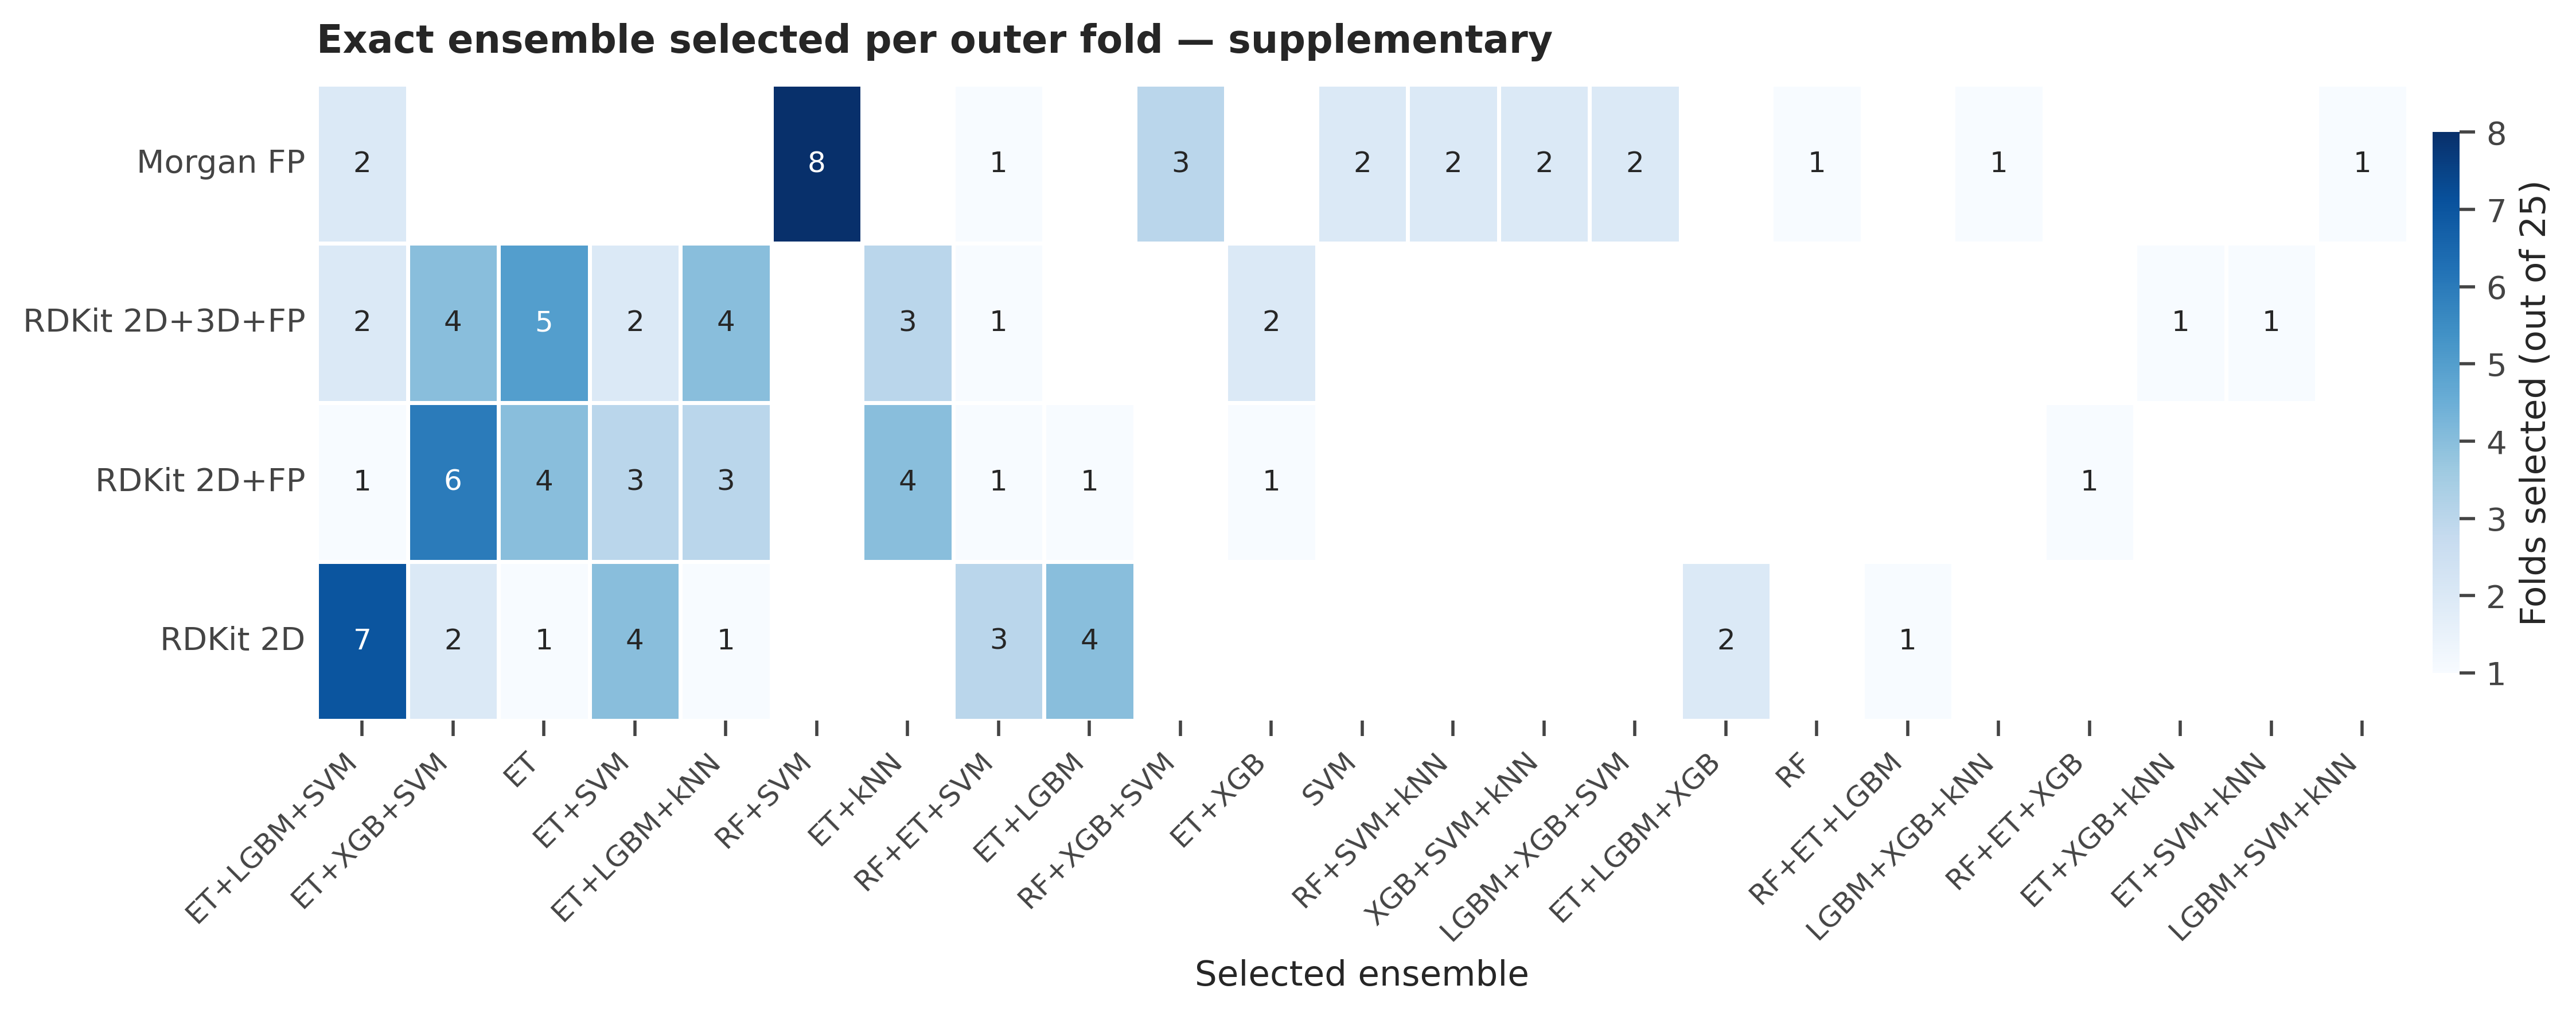
\includegraphics[width=\textwidth]{figures/S1_nested_cv_selection_full_heatmap.png}
	\caption{Stacking ensemble selected by the inner loop in each of the \TotalOuterFolds\ outer folds, for each molecular representation. Cell values are the number of outer folds in which that exact combination of base learners (RF, random forest; ET, extra trees; LGBM, LightGBM; XGB, XGBoost; SVM, support vector regression; kNN, $k$-nearest neighbors) was chosen. No combination was chosen consistently, which shows that the inner search does not converge on a single architecture.}
	\label{fig:selection_heatmap}
\end{figure}
